\chapter{Static program analysis}

Static code analysis is a field of computer science that studies algorithms for analyzing the program code. As opposed to dynamic code analysis that relies on executing the code and capturing information during the execution, the static analysis works on code without ever executing it. Techniques studied in this field are leveraged in today's optimizing compilers and specialized tools for verifying program correctness.

It is important to note that according to the Rice's theorem \citep{Rice1953} any non-trivial property of the program behavior in a Turing-complete language is undecidable. Thus most of the techniques outlined below compute only conservative approximate answers. The engineering challenge is to use a correct combination of the algorithms and to choose a correct approximation for a particular problem. Most of the methods outlined below could be implemented with different levels of precision at the cost of the analysis time. While it may be tempting to assume that the most precise method will always give the best answer it was shown before \citep{Milanova2002} that even less precise methods could lead to the best solutions.

The rest of this chapter is organized as follows. Section 3.1 describes the analysis of program metadata and defines class hierarchy graph. Section 3.2 describes the concepts behind intraprocedural analysis, specifically the control-flow graphs and data-flow analysis and shows how to implement them. Section 3.3 then extends the intraprocedural concepts to interprocedural level.

\section{Metadata analysis}

Metadata analysis is by far the cheapest static analysis that can be performed. It summarizes facts about program metadata, such as method and variable names, class hierarchy and other attributes.

In the context of .NET Framework the metadata analysis is widely used by tools like Gendarme, FxCop and Visual Studio Code Analysis to analyze programs and libraries for violation of naming conventions. Tools like .NET Reflector, ILSpy \citep{ILSpy} or Visual Studio Object Browser use metadata to allow browsing .NET assemblies. It also serves as a basis for more advanced analyses.

\subsection{Class hierarchy}
Class hierarchy analysis builds a graph that represents inheritance relationships of object types and interfaces in a program. Each vertex of the graph represents a single type. Edges represent a relation of inheritance or, in case of interfaces, implementation respectively.

The class hierarchy graph is useful for resolving dynamic calls to virtual or interface methods. Given a known type and a method reference it is possible to traverse the class hierarchy towards the leafs and find all implementations of the method.

\paragraph{Example} On Listing ~\ref{fig:classHierarchySource} we present a simple class hierarchy written in C\# code. The corresponding class hierarchy graph is shown on Figure ~\ref{fig:classHierarchyGraph}.

\begin{lstlisting}[language=CSharp,caption=C\# representation of type hierarchy,label=fig:classHierarchySource]
interface IFoo { }  
interface IBar : IFoo { }
class A { }
class B : A, IFoo { }
class C1 : B { }
class C2 : B { }
\end{lstlisting}

\begin{figure}[h]
\begin{center}
\digraph[scale=0.65]{ClassHierarchy}{
"IFoo" [style=dashed]
"IBar" [style=dashed]
"IFoo" -> "IBar";
"B" -> "A";
"B" -> "IFoo";
"C1" -> "B";
"C2" -> "B";
"A" -> "System.Object"
}
\caption{Class hierarchy graph}
\label{fig:classHierarchyGraph}
\end{center}
\end{figure}

\section{Intraprocedural analysis}

Control-flow and data-flow analyses form the foundation for many advanced static analyses. Both analyses are usually carried out on intermediate code representation (such as ECMA 335 Common Intermediate Language, Java byte code, GCC's GIMPLE or the Jimple representation of Java code). While it is possible to implement both of them on a higher-level representation, such as abstract syntax trees, it is often not beneficial because the analyses would have to deal with all the constructs of the source language. Implementations of the analyses on higher-level representation are mostly used by refactoring tools or tools for checking coding conventions that need access to details that would be lost by conversion to the intermediate representation.

We will first introduce concepts of these analyses on single method scope and the next section will explain how to modify them and use them for interprocedural analysis.

\subsection{Control-flow}

Control flow analysis is a method of analyzing a single method and building its control flow graph. 

To define a control-flow graph a basic block (also called elementary block) construct has to be introduced. A basic block is an ordered block of statements that are always executed sequentially, none of the statements is target of a branch and none of the statements, except for the last one, is a branch statement.

A control-flow graph is a directed graph $G(V, E, entrypoint)$, where all vertices $v \in V$ are statements of the method and $entrypoint \in V$ defines the entry statement of the method. There is an edge $e \in E$ between two statements $v_1, v_2 \in V$ if a control can flow from $v_1$ to $v_2$ (e.g. $v_2$ is a possible target of the branch statement in $v_1$ or $v_2$ is a sequentially executed statement). It is often beneficial to use storage representation where each vertex in the control-flow graph is a basic block since the control-flow within individual statements of basic blocks is always sequential, so the basic block graph is more compact. The resulting graphs are isomorphic.

\paragraph{Constructing a control-flow graph} for a single function is performed by traversing from entrypoint through all the statements sequentially and marking any statement that is a target of a branch or that itself is a branch statement. These marks then divide the function into several basic blocks that can be connected by making edges from the branch statements to the target blocks.

Several adjustments to the above algorithm have to be done to accompany the concept of exceptions. There are two common approaches to this problem. The first one builds the control-flow graph with edges that represent potential exception flows between the blocks \citep{Sinha2000}. The other approach builds a separate control flow graph for normal flow and exception flow, which seems to be a good enough approach for most static analyses and code patterns \citep{Jo_constructingcontrol}.

\subsection{Data-flow}

Data-flow analysis derives information about the dynamic behavior of a program by only examining the static code. It gathers information about possible set of values calculated at various program points. The control-flow graph is utilized for determining where to propagate the values between different program points.

There are several data-flow analyses that compute various program properties, such as the liveness analysis or reaching definitions analysis. All of the data-flow analyses have some common properties and can be modeled and computed using the same basic framework that will be presented in this section.

Each data-flow analysis has its defined problem domain, which is required to be finite in order to ensure that the analysis can be computed. It generates a symbolic \emph{in-state} and \emph{out-state} for each statement in the control flow graph. The states are defined within the problem domain. The in-state represents the state before the statement is executed and the out-state represents the state after the statement is executed. \emph{Flow equations} are defined that transfer an in-state into an out-state, or vice-versa, based on the statement. An initial in-state is defined for the method entrypoint, which we will refer to as an \emph{initial guess} (conversely an initial out-state is defined for method exitpoint(s) if the control-flow graph is traversed backwards).

We will first demonstrate how such analysis may look and what results will be produced and then generic framework will be presented that can be used for specifying and solving various data-flow problems.

\paragraph{Example} \emph{Liveness analysis} is one of the simplest data-flow analyses. The purpose of this analysis is to determine which variables are referenced beyond a particular program point. These variables are considered \emph{live} and form a subset of all the variables used in a given method. Motivation for this particular analysis is that the information is useful for register allocation in compilers, where the variables must be assigned to a limited number of registers. A register can be reused whenever it is known that the variable stored in it is not live beyond the particular program point.

Given the program in Figure ~\ref{fig:livenessProgram} we can calculate the live variables at each program point as shown in Figure ~\ref{fig:livenessResults}. The \emph{out} column in that table specifies the live variables after a given program point and the \emph{in} column shows the live variables before the statement at the program point. The particular method used to calculate the values will be explained later in this chapter.

The problem domain for liveness analysis are all the variables in the method, thus $|variables| \times |CFG\ vertices| \times 2$ values are computed. The control-flow graph is traversed backwards and the initial guess is empty set (ie. no variables are live beyond the method exitpoint). Flow function is shown in Listing ~\ref{fig:livenessEquations}.

\begin{lstlisting}[mathescape,caption=Flow equations for liveness analysis,label=fig:livenessEquations]
${\mbox{LIVE}}_{in}[s] = {\mbox{USE}}[s] \cup ({\mbox{LIVE}}_{out}[s] \setminus {\mbox{DEF}}[s])$
${\mbox{LIVE}}_{out}[s] = \bigcup_{p \in succ[s]} {\mbox{LIVE}}_{in}[p]$
${\mbox{LIVE}}_{out}[exitpoint] = {\emptyset}$  - Initial guess
${\mbox{DEF}}[s]$ - Set of variables that are defined in statement $s$
         (ie. a value is assigned to the variable)
${\mbox{USE}}[s]$ - Set of variables that are used in statement $s$
         (ie. a value is read from the variable)
\end{lstlisting}

\begin{figure}
\begin{center}
\digraph[scale=0.65]{LivenessProgram}{"1) a = 0" -> "2) b = a + 1" -> "3) c = c + b" -> "4) a := b * 2" -> "5) if a < 11 goto L2" -> "2) b = a + 1"; "5) if a < 11 goto L2" -> "6) return c"}
\caption{Sample method used for demonstration of liveness analysis}
\label{fig:livenessProgram}
\end{center}
\end{figure}

\begin{figure}
\begin{center}
\begin{tabular}{ l | c c | c c }
& use & def & out & in \\
\hline
6) & c & & & c \\
5) & a & & ac & ac \\
4) & b & a & ac & bc \\
3) & bc & c & bc & bc \\
2) & a & b & bc & ac \\
1) & & a & ac & c \\
\end{tabular}
\caption{Output of liveness analysis for the sample method}
\label{fig:livenessResults}
\end{center}
\end{figure}

\paragraph{Example} \emph{Reaching definitions} is a data-flow analysis which statically determines which definitions may reach a given point in the code. A definition is represented by a statement that defines a variable (it is assumed that each statement can define only one variable). The domain of values for the analysis is thus a set of statements of the analyzed method. In other words, each computed in- and out- state is a set of definition statements whose definition can reach the statement associated with the respective in- or out- state. Flow function for reaching definitions is shown in Listing ~\ref{fig:reachingDefinitionsEquations}.

The results of the analysis can be used for loop invariant motion (ie. moving code out of loops if it doesn't depend on variables defined inside the loop) or for computing the use-def chains and def-use chains. It is a canonical example of forward data-flow analysis.

\begin{lstlisting}[mathescape,caption=Flow equations for reaching definitions,label=fig:reachingDefinitionsEquations]
${\mbox{REACH}}_{\rm in}[s] = \bigcup_{p \in pred[s]} {\mbox{REACH}}_{\rm out}[p]$
${\mbox{REACH}}_{\rm out}[s] = {\mbox{GEN}}[s] \cup ({\mbox{REACH}}_{\rm in}[s] \setminus {\mbox{KILL}}[s])$
${\mbox{GEN}}[s : y \leftarrow f(x_1,\cdots,x_n)] = \{s\}$
${\mbox{KILL}}[s : y \leftarrow f(x_1,\cdots,x_n)] = {\mbox{DEFS}}[y] - \{s\}$
${\mbox{DEFS}}[y]$ - Set of all definition statements that assign to the variable $y$
\end{lstlisting}

\subsubsection{Computation of the data-flow analyses}

Flow equations together with the control-flow graph form a set of equations, where the two flow equations correspond to each control-flow graph vertex. For most data-flow analyses one of the flow equations is in form ${\rm IN}[S] = \bigcup_{p \in pred[S]} {\rm OUT}[p]$ or ${\rm OUT}[S] = \bigcup_{p \in succ[S]} {\rm IN}[p]$, the other is referred to as \emph{flow function} (also \emph{transfer function}). The first form is used by \emph{forward} data-flow analyses (such as Reaching definitions), which are computed by traversing the control-flow graph from entrypoint towards exitpoint(s). The second form is used by \emph{backward} data-flow analyses (such as Liveness analysis), which are computed by traversing the control-flow graph from exitpoint(s) towards the entrypoint.

For the rest of this section we will assume that the data-flow analysis is either forward or backward. Other types of analyses exist, which are neither forward nor backward, such as partial redundancy elimination, but they are uncommon. Moreover we will assume that all the algorithms that work for forward analysis can also be applied for backward analysis by substituting entrypoint for exitpoint(s), in-states for out-states, successors for predecessors in control-flow graph and vice-versa. The following text will cover only forward data-flow analysis and the principles for backward analysis can be trivially derived.

Computation of the data-flow analyses is straightforward for basic blocks in the control-flow graph. One just has to iterate over the statements and propagate the in- and out-states through the flow function. Likewise it is straightforward to compute the analysis for control-flow graphs that don't contain cycles, it is sufficient to traverse the graph in topological order. The complication is how to compute the information for loops and other forms of branches in control flow.

It was established that in order to define a specific data-flow analysis we have to define its problem domain, the direction of traversal of the control-flow graph, flow function, initial guess and a merge function. The next section will try to formalize these building blocks a bit and show how to compute the in- and out- states efficiently and how to deal with the problem of loops in the control-flow graph.

\subsubsection{Lattice framework}

\emph{Lattice framework} (also referred to as \emph{Monotone framework}) aims to provide a formal theoretical model that describes all the data-flow analyses. It then exploits the lattice theory to achieve various goals, such as defining the theoretical computational complexity. Only basics are explained in this thesis, for a full explanation we refer to \citet{Nielson1999}, \citet{Muchnick1998} and \citet{Aho1986}.

\begin{definition}
A \emph{partially ordered set} is a structure $L = (S, \sqsubseteq)$, where $S$ is a set and $\sqsubseteq$ is a binary relation that is reflexive, transitive and anti-symmetric.
\end{definition}

\begin{definition}
A \emph{lattice} is a partially ordered set in which any two elements have an unique supremum (elements' least upper bound, referred to as \emph{join} or $x \sqcup y$) and unique infimum (greatest lower bound, referred to as \emph{meet} or $x \sqcap y$). Furthermore, a \emph{bounded lattice} must have an unique largest element $\top = \sqcup S$ and unique smallest element $\bot = \sqcap S$.
\end{definition}

\begin{definition}
Every finite set $A$ defines a \emph{powerset lattice} $(2^A, \subseteq)$, where $\bot = \emptyset$, $\top = A$, $x \sqcup y = x \cup y$, $x \sqcap y = x \cap y$. The height of such a lattice is the longest path from $\bot$ to $\top$, thus $|A|$.
\end{definition}

The problem domain is organized into a lattice. Each element of  the lattice corresponds to one possible value of an in- or out-state, also referred to as \emph{flow value}. The value $\bot$ represents the ``worst-case" information (eg. the universal set), $\top$ represents the ``best-case" information (eg. the empty set). If $x < y$ then $x$ is a conservative approximation of $y$. Flow function $F(statement, v): v \rightarrow v'$  maps the program behavior onto the lattice $V$ for $v, v' \in V$. The merge function is defined using the lattice operators as either meet or join.

Complex problem domains can be described by an $n$-tuple of lattices. Product of the lattices in the $n$-tuple also forms a lattice. An example is shown in Figure ~\ref{fig:latticeTuples}.

At each program point we strive to compute the flow values by considering all the paths leading from the entrypoint to a particular program point and then merging these values together. This concept is called \emph{meet-over-all-paths} (MOP). This is impossible to compute for loops, where the number of paths leading to a program point is infinite. The solution is to compute the merges early at merge point by computing the \emph{maximum fixed point} (MFP). Computing the flow values at merge points is only legal if the flow function $F$ is monotone. It is then provable that flow values computed have the following relation: $MFP \leq MOP \leq ideal\ solution$. Furthermore, if the flow function $F$ distributes over the merge operator (meet or join) then solutions computed by MFP and MOP are equivalent.

% A framework (F, V, ?) is monotone iff x ? y implies f(x) ? f(y)
% Equivalently, a framework (F, V, ?) is monotone iff  f(x ? y) ? f(x) ? f(y), meet inputs, then apply f ? apply f individually to inputs, then meet results 

\begin{figure}
\begin{center}
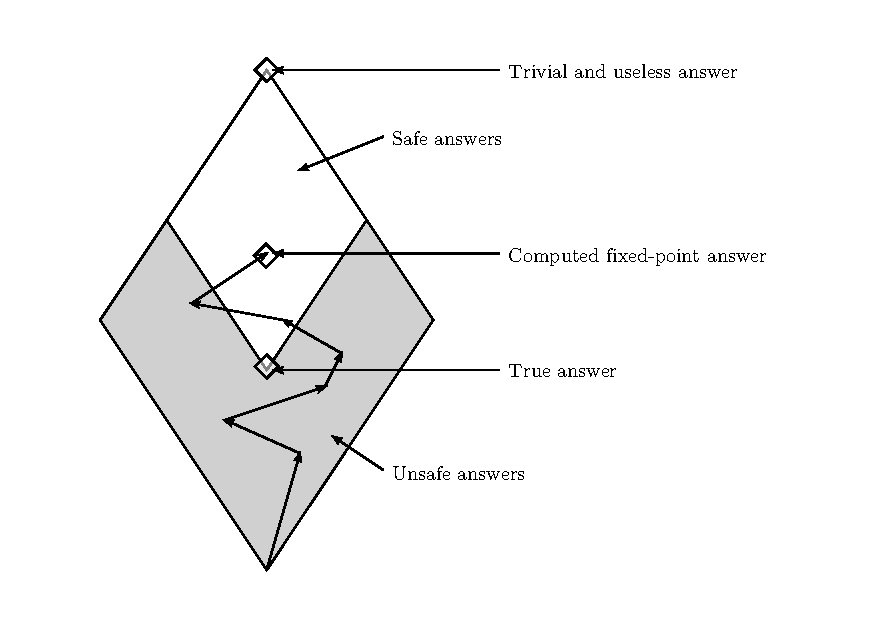
\includegraphics[scale=0.85]{LatticeAnswers.pdf}
\caption{Lattice points as answers \citep{Schwartzbach2009}}
\end{center}
\end{figure}

\paragraph{Example} Given the example of the liveness analysis we can see that the problem domain is a set of all the variables that can occur at each program point. If the set of variables was ${a, b, c}$ then the corresponding lattice would look like that in Figure ~\ref{fig:livenessLattice}.

\begin{figure}
\begin{center}
\graph[scale=0.65]{Lattice}{
"{a,b,c}" -- "{a,b}"
"{a,b,c}" -- "{a,c}"
"{a,b,c}" -- "{b,c}"
"{a,b}" -- "{a}"
"{a,c}" -- "{a}"
"{a,b}" -- "{b}"
"{b,c}" -- "{b}"
"{a,c}" -- "{c}"
"{b,c}" -- "{c}"
"{a}" -- "{}"
"{b}" -- "{}"
"{c}" -- "{}"
}
\caption{Subset lattice for a set of three variables}
\label{fig:livenessLattice}
\end{center}
\end{figure}

\begin{figure}
\begin{center}
\subfloat[$X$]{ \graph[scale=0.65]{LatticeTuples1}{"{}" -- "{a}"} }
\subfloat[$Y$]{ \graph[scale=0.65]{LatticeTuples2}{"{}" -- "{b}"} }
\subfloat[$X \times Y$]{ \graph[scale=0.65]{LatticeTuples3}{"{},{}" -- "{a},{}" -- "{a},{b}"; "{},{}" -- "{},{b}" -- "{a},{b}"} }
\caption{Product of two lattices ($\langle x_1, y_1 \rangle \leq \langle x_2, y_2 \rangle$ iff $x_1 \leq x_2$ and $y_1 \leq y_2$)}
\label{fig:latticeTuples}
\end{center}
\end{figure}

\subsubsection{Computing the fixed-point}

Computing the in- and out-states uses a simple idea that it is only necessary to recompute the out-state if the in-state has changed. The in-state can only change if out-state of any predecessors has changed, or in other words, if the out-state has changed then any successors will have to be recomputed. The generic algorithm for computing the data-flow analysis exploits this fact. Initially all the in-states are initialized to $\emptyset$, except for the one corresponding to the entrypoint, which is initialized to the initial guess. A work list is used to keep a track of all vertices in a control-flow graph for which the in- and out-states have to be recomputed. The work list is initialized with the entrypoint vertex at first. The work list is then processed until it is empty. In each iteration one out-state is computed and all the successors are added to the list for recomputing if the out-state differs from the one computed earlier or if it is the first computed out-state for the particular vertex.

\begin{myalgorithm}
\caption{Computing data-flow analysis using work-list}
\begin{algorithmic}
\FORALL {$v \in Vertices$}
	\STATE $in[v] \gets \emptyset$
	\STATE $out[v] \gets \emptyset$
\ENDFOR
\STATE $in[entry\ vertex] = initial\ guess$
\STATE $worklist = \{entry\ vertex\}$
\WHILE {$worklist \neq \emptyset$}
	\STATE $v \gets deque(worklist)$
	\STATE $out' \gets out[v]$
	\STATE $in[v] \gets \cap out[p]\ for\ all\ p \in predecessor(v)$
	\STATE $out[v] \gets Transfer(in[v], v)$
	\IF {$out[v] \neq out'$}
		\FORALL {$s \in successors(v)$}
			\IF {$s \notin worklist$}
				\STATE $enqueue(worklist, s)$
			\ENDIF
		\ENDFOR
	\ENDIF
\ENDWHILE
\end{algorithmic}
\end{myalgorithm}

\subsubsection{Classification}

\paragraph{May-analysis} identifies possibilities and gathers information that answers whether a specific condition may happen in some code path. It's usually implemented with an initial guess being empty set, a merge function that produces union of the sets (ie. join) and a flow function that adds all possibilities to the set and removes only those possibilities that are guaranteed not to be false.

\paragraph{Must-analysis} provides a guarantee and gathers information that answers whether a specific condition must happen in all code paths. It's usually implemented with an initial guess being empty set, a merge function that produces intersection of the sets (ie. meet) and a flow function that adds only those possibilities that are guaranteed to be true and removes any possibilities that may not happen.

\paragraph{Path-sensitive} analyses use branch conditions and assume that the condition is true on the path if the branch is taken and analogously it is assumed that the condition is false on the path if the branch is not taken. The algorithm for computing the path-sensitive analyses is slightly different from the one presented here and is not covered by this paper.

\section{Interprocedural analysis}

Modern programming languages allow structuring the program code into methods (procedures or functions) that call each other and separate the functionality of the program into isolated chunks. Thus intraprocedural analysis is often not satisfactory for any complex program analysis and serves only as a building block for interprocedural analysis that analyses the program globally.

While the basic algorithm principles are similar for intraprocedural and interprocedural analysis the explored state space is much larger and thus most of the algorithms for interprocedural analyses are about making compromises between accuracy and required computational time.

\subsubsection{Classification}

\paragraph{Flow-sensitive} analyses compute one answer for every program point. It requires intraprocedural data-flow analysis or similar technique. \emph{Flow-insensitive} analysis ignores control-flow and computes one answer for every method. Flow-insensitive analysis is less accurate than the flow-sensitive one, but it can be computed in linear time. There are problems that can be answered adequately with a flow-insensitive analysis, such as whether variable $x$ can be modified by a given method.

\paragraph{Context-sensitive} analyses distinguishes between different call sites of methods. Computing a context-sensitive analysis efficiently is still subject of current research and there are various methods to do it. The simplest approach is to reanalyze callee for each caller, which is often very expensive. Another approach is to compute a generic intraprocedural analysis for each method and then specialize the computed summary for each call site \citep{Gulwani2007}. Yet another technique that is often used are \emph{$k$-context-sensitive algorithms} \citep{Shivers1991,Might2007}, which distinguish call sites up to $k$ levels deep in the call graph and then rerun the callee analysis for each different call site chain. Figure ~\ref{fig:contextSensitivity} shows an example of values gathered by context-sensitive and context-insensitive analyses.

\begin{figure}
\begin{center}
\subfloat[Context-sensitive]{\digraph[scale=0.65]{ContextSensitive}{
   "a = id(4);" -> "id(x) { return x; }" [label="  "];
   "b = id(5);" -> "id(x) { return x; }" [label="  "];
   "id(x) { return x; }" -> "a = id(4);" [label=" 4 ", style=dashed];
   "id(x) { return x; }" -> "b = id(5);" [label=" 5 ", style=dashed];
}}
\subfloat[Context-insensitive]{\digraph[scale=0.65]{ContextInsensitive}{
   "a = id(4);" -> "id(x) { return x; }" [label="  "];
   "b = id(5);" -> "id(x) { return x; }" [label="  "];
   "id(x) { return x; }" -> "a = id(4);" [label=" 4, 5 ", style=dashed];
   "id(x) { return x; }" -> "b = id(5);" [label=" 4, 5 ", style=dashed];
}}
\caption{Difference between context-sensitive and context-insensitive analysis. Context-sensitive analysis provides different answer for a method depending on the context it is called in. Context-insensitive analysis gives a same summary answer for a method regardless of the specific context it is called in. The summary answer is true for all possible calling contexts of the method.}
\label{fig:contextSensitivity}
\end{center}
\end{figure}

\paragraph{Path-sensitive} interprocedural analysis computes one answer for each possible execution path. This is approach taken by model checkers and it is extremely expensive both in terms of memory and computational resources. While many techniques were developed to reduce the searched state space the path-sensitive analysis is still not practical for whole program analysis.

\paragraph{Top-down and bottom-up} Similarly to forward and backward intraprocedural data-flow analysis the graph in interprocedural analysis can be processed in several orders. The \emph{bottom-up} order starts at the leaf methods and summarizes effects of called methods for callers. Conversely the \emph{top-down} order starts at the root methods and summarizes effects of caller for callees.

\subsection{Call graph}

\emph{Static call graph} (also referred to as Procedure Call Graph or PCG) is a directed graph that represents calling relationships between methods in a computer program. For a program with methods $(m_1...m_n)$ the static call graph is defined as $G = (V, S, E, entrypoint)$, where $V = (m_1...m_n)$, $S$ is set of call site labels (ie. labels of program points where a call is performed), $E \subseteq V \times V \times S$ and $entrypoint \in V$ being the program entrypoint.

Construction of a call graph is trivial for languages that don't feature dynamic dispatch (ie. virtual methods in object oriented languages, function pointers or other forms of indirect calls). For languages with dynamic dispatch, such as Java or C\#, computing a static call graph precisely requires alias analysis results. Conversely, computing precise aliasing requires a call graph. To solve this problem both alias analysis and call graph construction have to be performed simultaneously.

An over-approximated call graph can be computed trivially even for languages with dynamic dispatch by employing various techniques, such as resolving virtual method calls using the class hierarchy graph based on declared variable type. We will refer to this over-approximation as \emph{CHA call graph}. A simple extension of this approach is the \emph{Rapid-Type Analysis} \citep{Bacon1997}, where the CHA call graph is reduced by using the fact that an instance method cannot be called unless the type is instantiated in the program.

\subsection{Data-flow}

There are several methods for computing data-flow analyses on interprocedural level. The most fundamental ones will be explored in this section, but unlike intraprocedural analysis there is no single canonical algorithm.

\subsubsection{Control-flow super graph}

\emph{Control-flow super graph} is constructed by combining control-flow graphs of all the methods into one huge graph by adding edges between call site and method entrypoint and exitpoint(s). The advantage of this representation is that intraprocedural data-flow analysis can be used unmodified on the super graph. It's not very practical though, because the performance of the work-list data-flow computation dependents directly on the number of cycles in the graph and each call site adds one cycle to the super graph. Also the super graph smears information from different contexts and thus such data-flow analysis would be context-insensitive.

\begin{figure}
\begin{center}
\digraph[scale=0.65]{ControlFlowSuperGraph}{
  subgraph cluster_foo {
    "x = 3" -> "bar(x)" -> "bar(1)"
    label="foo"
  }
  subgraph cluster_bar {
    "y = x + 1" -> "return"
    label="bar"
  }
  "bar(x)" -> "y = x + 1"
  "return" -> "bar(x)"
  "bar(1)" -> "y = x + 1"
  "return" -> "bar(1)"
}
\caption{Example of a control-flow super graph}
\label{fig:controlFlowSupergraph}
\end{center}
\end{figure}

\subsubsection{Invocation graph}

A brute-force approach for computing interprocedural data-flow analysis is to use an \emph{invocation graph} (Figure ~\ref{fig:invocationGraph}), where a distinct path exists for each possible call chain. It is inherently context-sensitive and also very precise, but due to the nature of the invocation graph it is also exponentially expensive in relation to program size and it is problematic to compute the analysis for recursive call chains. 

\begin{figure}
\begin{center}
\subfloat{
\parbox[b]{50mm}{
main() \{ foo(4); foo(5); \} \\
foo(x) \{ bar(x); \} \\
bar(x) \{ ... \} \\ \\ \\
}
\subfloat{
\digraph[scale=0.65]{InvocationGraph}{
foo2 [label="foo"]
bar2 [label="bar"]
main -> foo -> bar
main -> foo2 -> bar2
}
}
}
\caption{Example of an invocation graph}
\label{fig:invocationGraph}
\end{center}
\end{figure}

%\subsubsection{Partial transfer function}

%A \emph{partial transfer function} (PTF) describes the behavior of a method assuming that certain properties hold in the context where it is called. It can be reused in many calling contexts as long as the properties of the inputs to the method are the same. It was demonstrated for alias analysis that by precomputing a single partial transfer function for each method a fully context-sensitive analysis can be implemented efficiently \citep{Wilson1995}.

%  [Wilson et al'95]
% Use memoization.
% funcOutput = PTF(funcInput).
% PTF computed once for an "input pattern".
% Lazily compute PTFs for each procedure.

\subsubsection{Static call graph}

Interprocedural analysis can be computed directly on the static call graph by decoupling the intraprocedural part from the interprocedural part. The work-list algorithm that is used for computing the intraprocedural analysis is reused for traversing the static call graph. At each vertex an intraprocedural analysis is performed to compute a method summary, which is then merged back into the caller's symbolic state (Figure ~\ref{fig:StaticCallGraphUpdates}).

\begin{figure}
\begin{center}
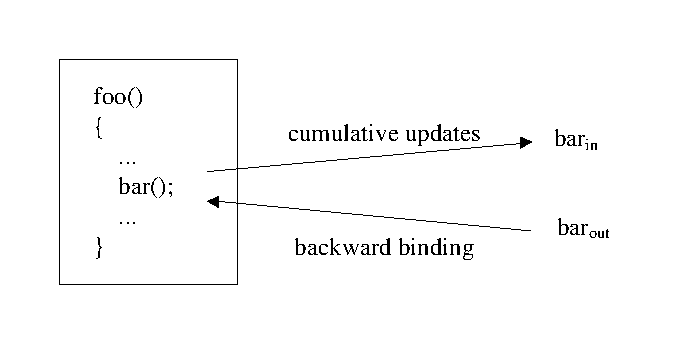
\includegraphics[scale=0.8]{StaticCallGraphUpdates.pdf}
\end{center}
\caption{Updates in an interprocedural analysis on static call graph. The calling context summary, represented by $bar_{in}$ is union of all possible in-states at all call sites of $bar$. The method summary, represented by $bar_{out}$, is computed by intraprocedural analysis of $bar$ with the initial guess $bar_{in}$. It is merged back into the out-state at each call site of $bar$.}
\label{fig:StaticCallGraphUpdates}
\end{figure}

% Procedure call graph [Choi et al'93]
% Each procedure - a PCG vertex.
% Each call site - an edge in PCG.

% Context insensitive.

The basic algorithm for computing the data-flow analysis on a static call graph is outlined in Algorithm ~\ref{fig:DataFlowPCG}. We show an iterative algorithm for simplicity, in practice the work-list algorithm is used. The flow function in the intraprocedural analysis has to be modified to account for calls by lazily reevaluating them using the values computed on the static call graph. The initial guess for the intraprocedural analysis is substituted with union of all in-states leading to the called method. 

\begin{myalgorithm}
\caption{Computing data-flow analysis on PCG}
\label{fig:DataFlowPCG}
\begin{algorithmic}
\REPEAT
	\FORALL {vertices $p \in PCG$}
		\STATE \COMMENT{Perform intraprocedural analysis, in this case a flow-insensitive one}
		\REPEAT
			\FORALL {vertices $n \in p.CFG$}
				\IF {statement $n$ is a call to $m$}
					\STATE Compute $n_{out}$ using $m_{out}$ and $n_{in}$
				\ELSE
					\STATE $n_{out} \gets F(n_{in})$
				\ENDIF
			\ENDFOR
		\UNTIL {for each vertex $n \in p.CFG$, $n_{in}$ and $n_{out}$ converge}

		\STATE \COMMENT{Construct the method summary}
		\STATE $p_{out} \gets$ merge of all $out$ flow values from exitpoints of $p$
		\STATE \COMMENT{Update the in-state for all called methods}
		\FORALL {methods $m$ called by $p$}
			\STATE $m_{in} \gets m_{in} \sqcup n_{in}$
		\ENDFOR
	\ENDFOR
\UNTIL {for each vertex $p \in PCG$, $p_{in}$ and $p_{out}$ converge}
\end{algorithmic}
\end{myalgorithm}

\begin{figure}
\begin{center}
\subfloat{
\parbox[b]{50mm}{
main() \{ foo(4); foo(5); \} \\
foo(x) \{ bar(x); \} \\
bar(x) \{ ... \} \\ \\ \\
}
\subfloat{
\digraph[scale=0.65]{ProcedureCallGraph}{
main -> foo -> bar
main -> foo
}
}
}
\caption{Example of a procedure call graph}
\label{fig:procedureCallGraph}
\end{center}
\end{figure}

\subsubsection{Static call graph with context-sensitivity}

The algorithm we presented in previous section can be modified to provide context-sensitivity \citep{Chatterjee1999,Cheng2000}. Instead of computing a method summary based on a specified initial guess we construct a \emph{context independent summary function} (CISF). The intraprocedural analysis computes a symbolic summary with unknown initial guess that can be transferred by the CISF for a specific context it is called in.

\subsection{Alias analysis}

Languages that support pointers or references introduce a complication for static analysis. Two (or more) variables may refer to the same memory location at the same time. A pessimistic assumption that two variables may always point to the same location is sound, but often hinders the particular analysis to the point that it is ineffective. A slightly better assumption that can be made for many languages is that two variables may alias if they are declared to be the same type or if they can be casted to a common parent type or interface.

Additional complication are objects created on the heap. There is a potentially unbounded number of them and so in order to be able to reason about them we have to represent them using a bounded approximation. One such approximation is to use the allocation site (ie. program point of the allocation, possibly together with call site for context-sensitive algorithms).

\emph{Alias analysis} is a static analysis that computes information about possible aliases for variables, which in effect helps other analyses make less conservative decisions.

The best known flow-based alias analyses are described by \citet{Andersen1994} and \citet{Steensgaard1996}, which are briefly described below.

\begin{figure}
\begin{center}
\unitlength 1mm % = 2.845pt
\linethickness{0.4pt}
\begin{picture}(80,60)(0,0)
\put(5,5){\vector(0,1){55}}
\put(5,5){\vector(1,0){75}}
\put(19,16){\oval(28,6)[]}
\put(19,16){\makebox(0,0)[cc]{Steensgard '96}}
\put(23,10){\oval(26,6)[]}
\put(23,10){\makebox(0,0)[cc]{Andersen '94}}
\put(40,30){\oval(20,6)[]}
\put(40,30){\makebox(0,0)[cc]{Burke '95}}
\put(65,30){\oval(20,6)[]}
\put(65,30){\makebox(0,0)[cc]{Choi '93}}
\put(60,55){\oval(22,6)[]}
\put(60,55){\makebox(0,0)[cc]{Emami '94}}
\put(69,49){\oval(22,6)[]}
\put(69,49){\makebox(0,0)[cc]{Wilson '95}}
\put(40,2){\makebox(0,0)[cc]{Flow-sensitivity}}
\put(2,30){\makebox(0,0)[cc]{\begin{sideways}Context-sensitivity\end{sideways}}}
\end{picture}
\caption{Overview of various alias analyses}
\label{fig:aliasOverview}
\end{center}
\end{figure}

\subsubsection{Representation}

There are several commonly used representations for the aliasing information. The following code written in C notation will be used as an example: $q=\&p; p=\&i; r=\&i;$.

\begin{itemize*}

\item \emph{Complete alias pairs} \citep{Landi1992} store all alias pairs explicitly. Example: $\langle*q, p\rangle, \langle*p, i\rangle, \langle*r, i\rangle, \langle**q, p\rangle, \langle**q, i\rangle, \langle*p, *r\rangle, \langle**q, *r\rangle$

\item \emph{Compact alias pairs} \citep{Choi1993} store only basic aliasing pairs. The complete aliasing pairs are derived using dereferencing, transitivity and commutativity. Example: $\langle*q, p\rangle, \langle*p, i\rangle, \langle*r, i\rangle$

\item \emph{Points-to relations} \citep{Emami1993} indicate that one variable points to another. Example: $(q, p), (p, i), (r, i)$

\end{itemize*}

\subsubsection{Steensgaard's analysis}

Steensgaard alias analysis has the following characteristics:
\begin{itemize*}
\item The algorithm is context-insensitive and flow-insensitive.
\item One points-to set is computed per pointer variable (eg. method argument, local variable, static field or instance field) over the entire program.
\item Pointer assignment is represented by unification constraints ($p = q$ implies $points\mhyphen{}to(p) = points\mhyphen{}to(q)$).
\item Fast union-find data structure is used for implementation. 
\item Solution is computed in almost linear time in terms of program size.
\item Imprecision stems from merging points-to sets.
\end{itemize*}
The general outline of the algorithm is the following:
\begin{itemize*}
\item Find all pointer assignment statements in the program.
\item Form points-to set $\{p\}$ for each pointer variable $p$.
\item Examine each assignment statement (eg. explicit assignment or implicit assignment during parameter passing), in an arbitrary order, and merge points-to sets for the involved variables.
\end{itemize*}

\subsubsection{Andersen's analysis}

Andersen's analysis offers more precision than Steensgard's analysis. It shares the context- and flow-insensitiveness characteristic. Pointer assignment is represented by inclusion constraints ($p = q$ implies $points\mhyphen{}to(p) \subseteq points\mhyphen{}to(q)$). The computed points-to graph is larger than Steensgaard's, but more precise. The analysis has in the worst case cubic complexity in terms of program size.

\subsubsection{FA analysis}

FA alias analysis is very similar to the Steensgaard's analysis. It is also computed using the union-find data structure, but compared to the Steensgaard's analysis it distinguishes between individual structure fields. The importance of the FA analysis lies in the fact, shown by \citet{Milanova2002}, that even though the analysis is relatively imprecise it yields sufficiently precise results for constructing call graphs of programs containing function pointers.
